
\documentclass[12pt]{article}

\usepackage[utf8]{inputenc}
\usepackage[bulgarian]{babel}
\usepackage{graphicx}
\usepackage{sidecap}  %required for side captions
\usepackage{amssymb}
\usepackage{amsmath}
\usepackage{hyperref}
\usepackage{commath}  
\usepackage{listings}
\usepackage[top=1.3in, bottom=1.5in, left=1.3in, right=1.3in]{geometry}


\begin{document}
	\begin{center}
        \LARGE{\textbf{Тема: Архитектура за класификация и съхранение на снимки, посредством ползване на услугите Amazon Rekognition, Amazon Lambda и Amazon CloudWatch}}
        
        \bigskip
        \Large{Предмет: Приложно-програмни интерфейси за работа с облачни архитектури с Амазон Уеб Услуги (AWS)}
        
        \medskip
        \Large{Изготвил: Венета Кирева, фн: 82184, имейл: fn82184@g.fmi.uni-sofia.bg}
        
        \medskip
        \Large{Лектор: проф. д-р Милен Петров, година: 2022/2023}
        
        \bigskip
	\end{center}
    
    
  %  \newpage
    \tableofcontents
    \bigskip
    \bigskip
    \newpage
  
\section{Условие} 

\hspace{\parindent}Създайте функционалност или архитектура, използвайки услугите на Amazon Web Services.

\section{Въведение}

\hspace{\parindent}Настоящият проект представя изграждането на архитектура в AWS за класификация и съхранение на изображения. За реализацията са използвани седем от услугите, предоставени от Amazon Web Services, като необходимите функционалности са в рамките на AWS Free Tier.

\clearpage
\pagebreak

\section{Теория}

\hspace{\parindent} Изображенията биват получени в 64-битов формат чрез Amazon SQS Queue. Чрез график, зададен в Amazon CloudWatch Event, през определени интервали от време се извиква Amazon Lambda Function, която декодира снимката и извиква Amazon Recognition, за да определи дали в нея е открит човек. Ако е открит, резултатот от изпълнението на Amazon Recognition в Amazon DynamoDB Table, а снимката запазва в Amazon S3 Bucket. Изпраща връзка за достъп до снимката, валидна 24 часа, до имейл адресите на абонираните потребители. 

\hspace{\parindent} 

\begin{figure}[h!]
\centering
    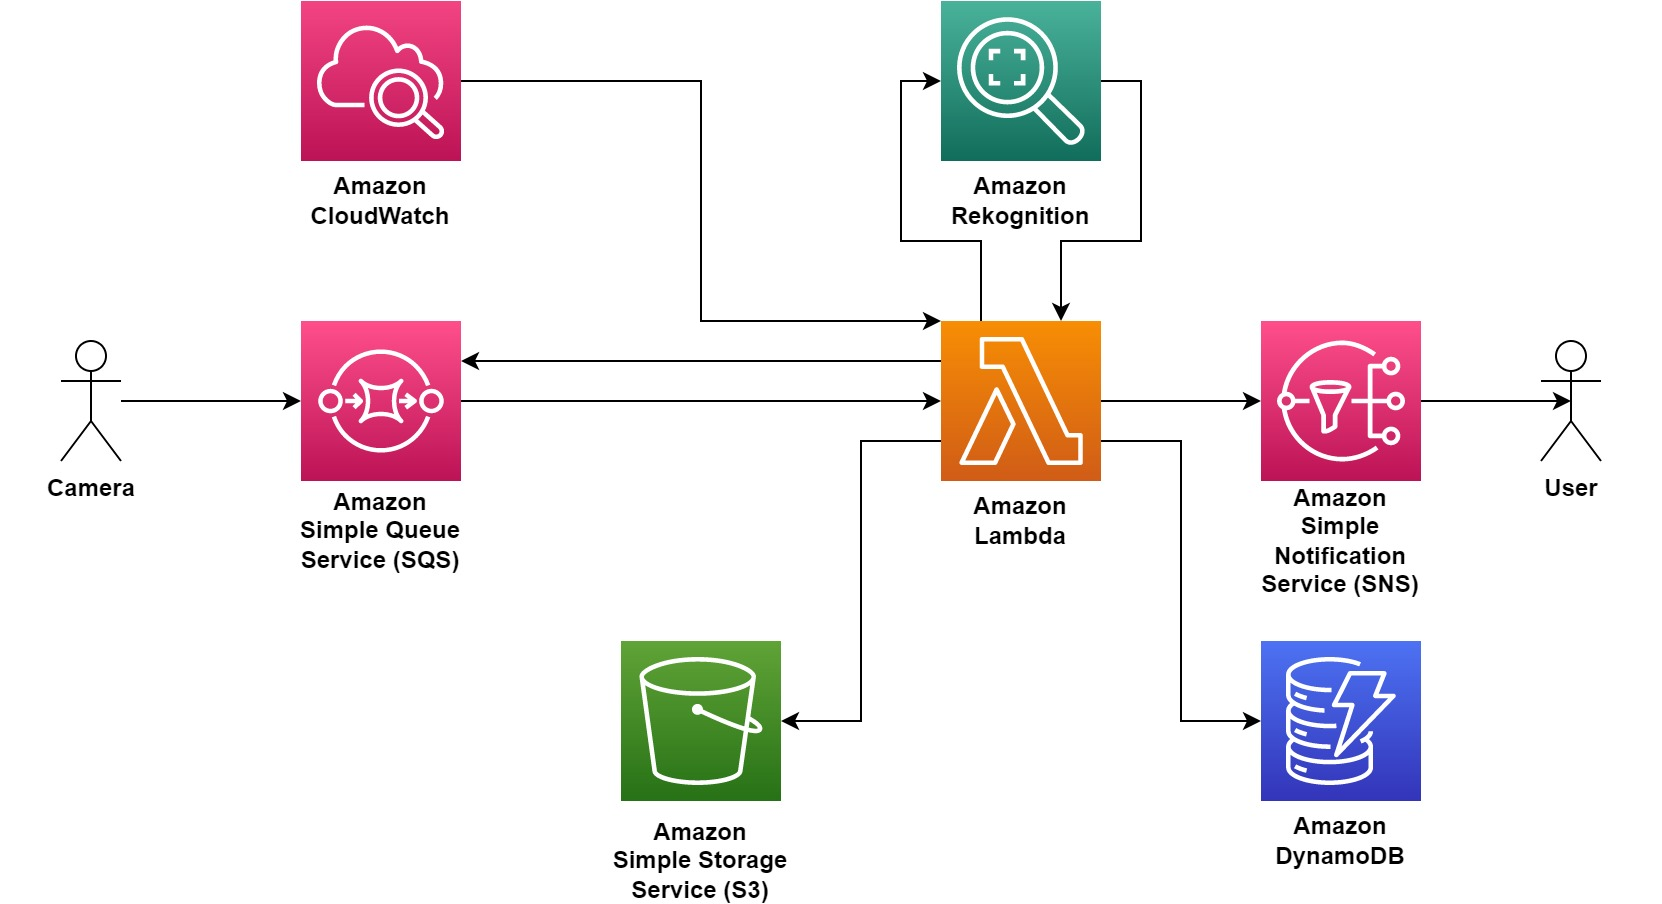
\includegraphics[width=\linewidth]{AWS_overview.jpg}
  \caption{Общ преглед на връзките между услугите. [Diagrams.net]}
\end{figure}

Веднъж на 24 часа информацията от Amazon DynamoDB Table се експортира в CSV файл и се запазва в Amazon S3 Bucket. На всеки 7 дни се изпраща имейл до абонираните потребители с напомняне за последния генериран CSV файл и връзка за достъп към него.

\begin{figure}[h!]
\centering
    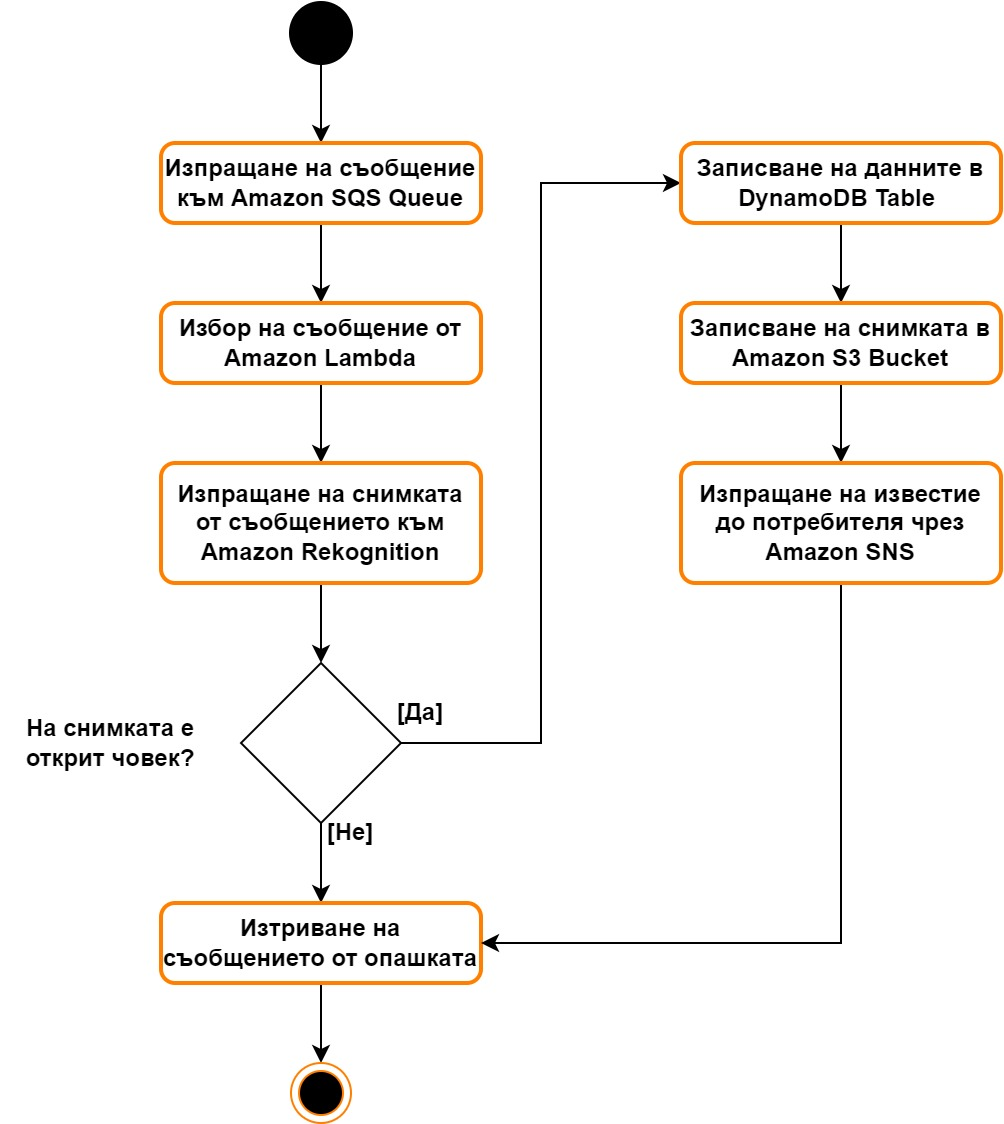
\includegraphics[width=\linewidth]{AWS_pic_process.jpg}
  \caption{Диаграма, показваща действията за обработване на получена снимка. [Diagrams.net]}
\end{figure}

\clearpage
\pagebreak

\section{Използвани технологии}
\begin{itemize}
    \item \textbf{Amazon CloudWatch} - услуга, събираща и обработваща данни за състоянието на системата.

    \item \textbf{Amazon DynamoDB} - безсървърна NoSQL база от данни.

    \item \textbf{Amazon Lambda} - безсървърна изчислителна услуга.

    \item \textbf{Amazon Rekognition} - SaaS платформа, осигуряваща инструменти за използването на компютърно зрение за анализ на изображения и видео.

    \item \textbf{Amazon Simple Notification Service (SNS)} - уеб услуга, управляваща изпращането и получаването на съобщения до абонирани  клиенти или точки на обслужване.

    \item \textbf{Amazon Simple Queue Service (SQS)} - услуга за опашка от съобщения.
    
    \item \textbf{Amazon Simple Storage Service (S3)} - уеб услуга, осигуряваща съхранение на обекти.
\end{itemize}

\clearpage
\pagebreak

\section{Инсталация и настройки}
\textbf{\hspace{\parindent}Преди да започнете с настройките на услугите е необходимо да сте влезли в AWS Free Tier акаунт.}
\subsection{Създаване на Amazon Simple Storage Service (S3) Bucket}

\noindent\textbf{Стъпка 1.} Напишете в търсачката "S3" и изберете \textit{S3} от падащото меню с услуги.
\begin{figure}[h!]
\centering
    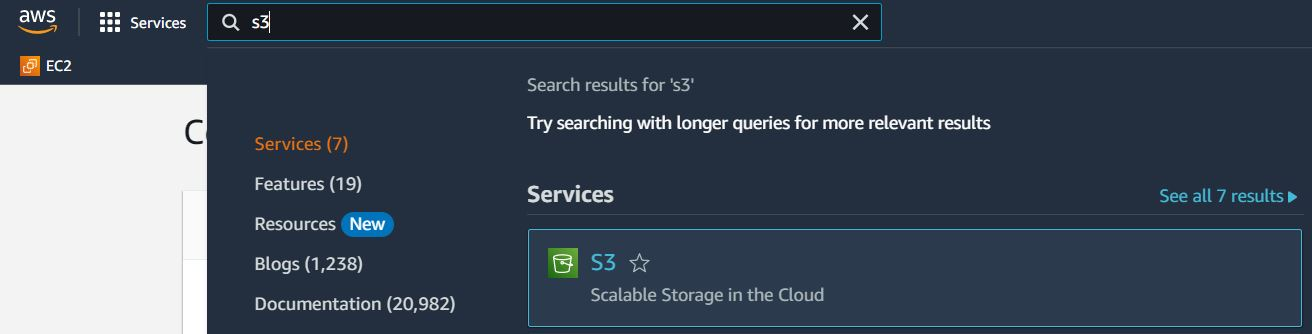
\includegraphics[scale=0.4]{instructions/s3/1.JPG}
  \caption{Създаване на Amazon S3 Bucket - стъпка 1.}
\end{figure}

\noindent\textbf{Стъпка 2.} От менюто изберете \textit{Buckets}.
\begin{figure}[h!]
\centering
    
\includegraphics[scale=0.55]{instructions/s3/2.JPG}
  \caption{Създаване на Amazon S3 Bucket - стъпка 2.}
\end{figure}

\noindent\textbf{Стъпка 3.} Изберете бутона \textit{Create bucket}.
\begin{figure}[h!]
\centering
    
\includegraphics[scale=0.6]{instructions/s3/3.JPG}
  \caption{Създаване на Amazon S3 Bucket - стъпка 3.}
\end{figure}

\noindent\textbf{Стъпка 4.} Попълнете в полето Bucket name име. За целите на текущото ръководство ще използваме \textbf{main-bucket}.
\begin{figure}[h!]
\centering
    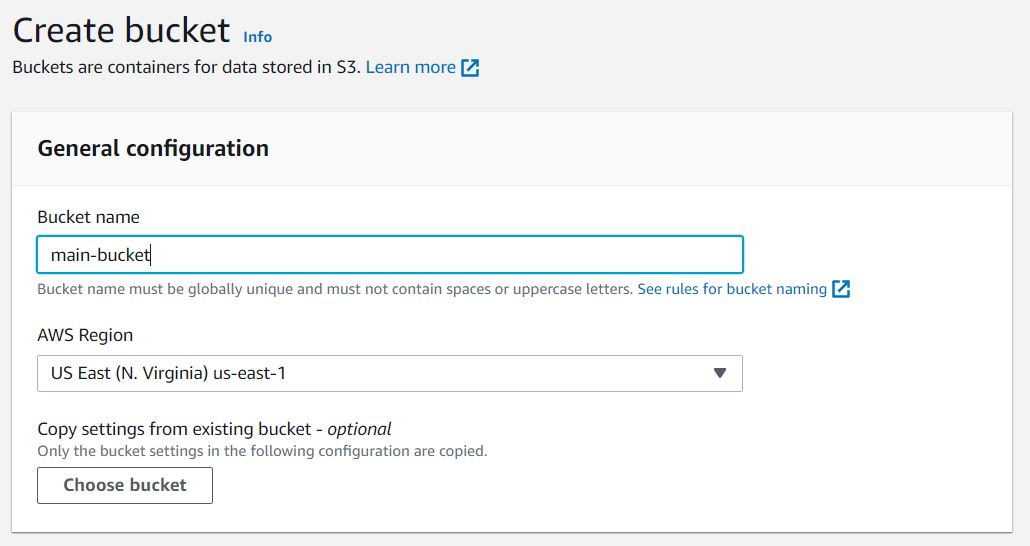
\includegraphics[scale=0.6]{instructions/s3/4.JPG}
  \caption{Създаване на Amazon S3 Bucket - стъпка 4.}
\end{figure}

\noindent\textbf{Стъпка 5.} Оставете настройките по подразбиране на останалите опции и изберете бутона \textit{Create bucket}.

\noindent\textbf{Стъпка 6.} Повторете отново стъпки 3. до 5. За целите на текущото ръководство за този AWS S3 Bucket ще използваме името \textbf{backup-bucket}.


\clearpage
\pagebreak

\subsection{Създаване на Amazon Simple Queue Service (SQS) опашка}
\noindent\textbf{Стъпка 1.} Напишете в търсачката "SQS" и изберете \textit{Simple Queue Service} от падащото меню с услуги.
\begin{figure}[h!]
\centering
    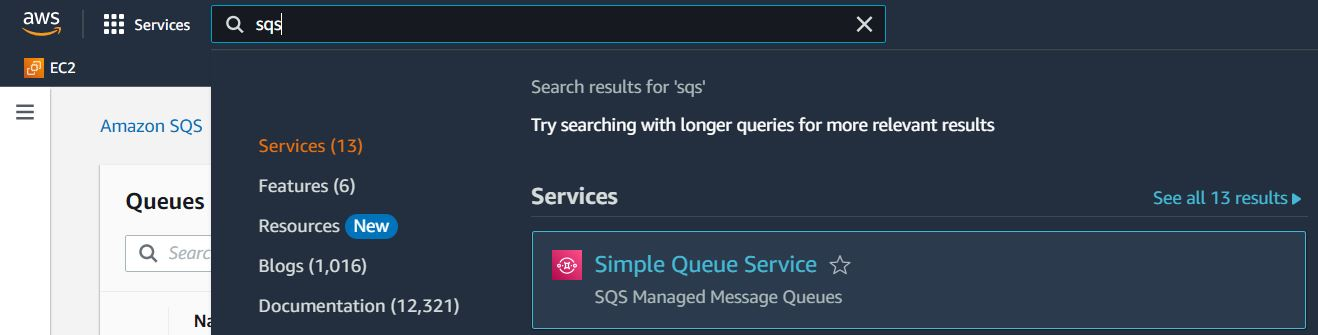
\includegraphics[scale=0.5]{instructions/sqs/1.JPG}
  \caption{Създаване на Amazon SQS опашка - стъпка 1.}
\end{figure}

\noindent\textbf{Стъпка 2.} Изберете бутона \textit{Create queue}.
\begin{figure}[h!]
\centering
    
\includegraphics[scale=0.55]{instructions/sqs/2.JPG}
  \caption{Създаване на Amazon SQS опашка - стъпка 2.}
\end{figure}

\noindent\textbf{Стъпка 3.} Попълнете в полето Name име. За целите на текущото ръководство ще използваме \textbf{queue}.
\begin{figure}[h!]
\centering
    
\includegraphics[scale=0.4]{instructions/sqs/3.JPG}
  \caption{Създаване на Amazon SQS опашка - стъпка 3.}
\end{figure}

\noindent\textbf{Стъпка 4.} Оставете настройките по подразбиране на останалите опции и изберете бутона \textit{Create queue}.

\clearpage
\pagebreak


\subsection{Създаване на Amazon DynamoDB таблица}
\noindent\textbf{Стъпка 1.} Напишете в търсачката "DynamoDB" и изберете \textit{DynamoDB} от падащото меню с услуги.
\begin{figure}[h!]
\centering
    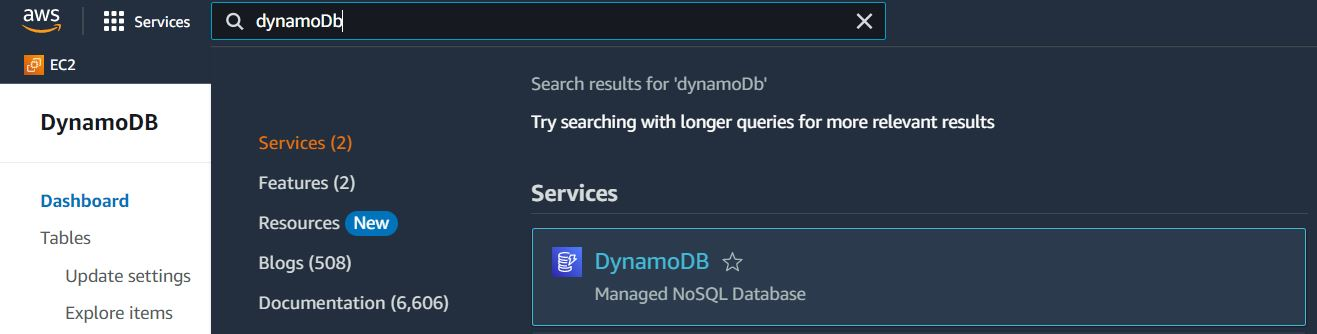
\includegraphics[scale=0.45]{instructions/dynamodb/1.JPG}
  \caption{Създаване на Amazon DynamoDB таблица - стъпка 1.}
\end{figure}

\noindent\textbf{Стъпка 2.} От менюто изберете \textit{Tables}.
\begin{figure}[h!]
\centering
    
\includegraphics[scale=0.55]{instructions/dynamodb/2.JPG}
  \caption{Създаване на Amazon DynamoDB таблица - стъпка 2.}
\end{figure}

\noindent\textbf{Стъпка 3.} Изберете бутона \textit{Create table}.
\begin{figure}[h!]
\centering
    
\includegraphics[scale=0.6]{instructions/dynamodb/3.JPG}
  \caption{Създаване на Amazon DynamoDB таблица - стъпка 3.}
\end{figure}

\noindent\textbf{Стъпка 4.} Попълнете в полето Name име. За целите на текущото ръководство ще използваме \textbf{table}. В полето Partition key въведете "picID".
\begin{figure}[h!]
\centering
    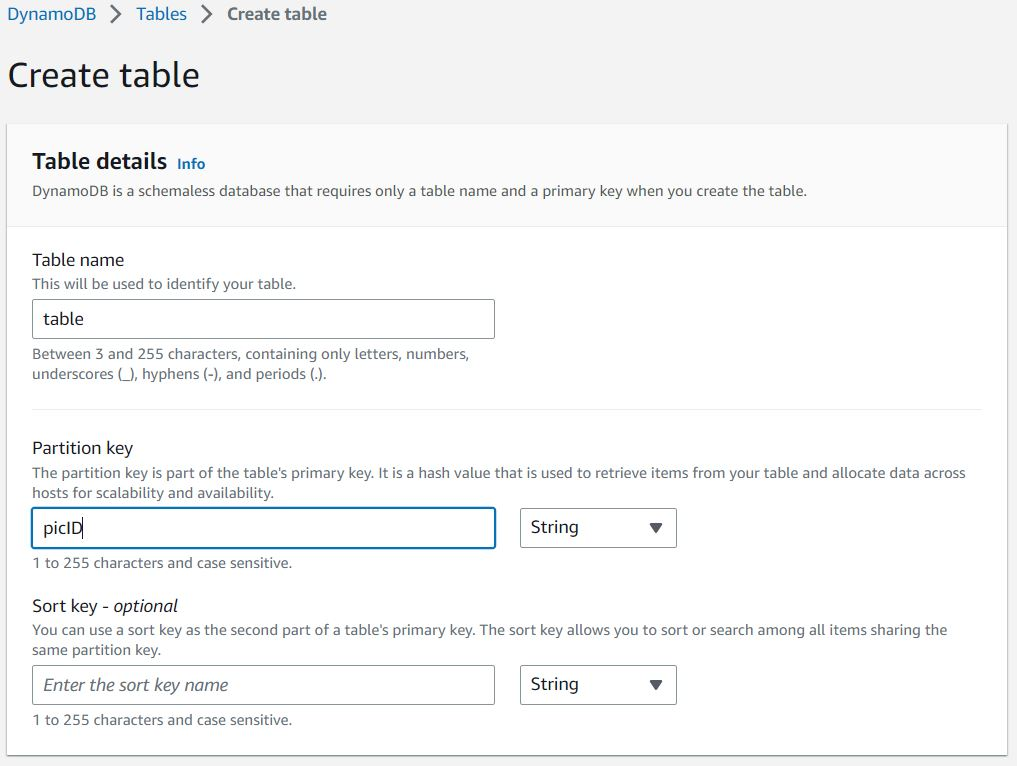
\includegraphics[scale=0.55]{instructions/dynamodb/4.JPG}
  \caption{Създаване на Amazon DynamoDB таблица - стъпка 4.}
\end{figure}

\noindent\textbf{Стъпка 5.} Оставете настройките по подразбиране на останалите опции и изберете бутона \textit{Create table}.

\clearpage
\pagebreak

\subsection{Създаване на Amazon Simple Notification Service (SNS) Topic и Subscription}
\noindent\textbf{Стъпка 1.} Напишете в търсачката "SNS" и изберете \textit{Simple Notification Service} от падащото меню с услуги.
\begin{figure}[h!]
\centering
    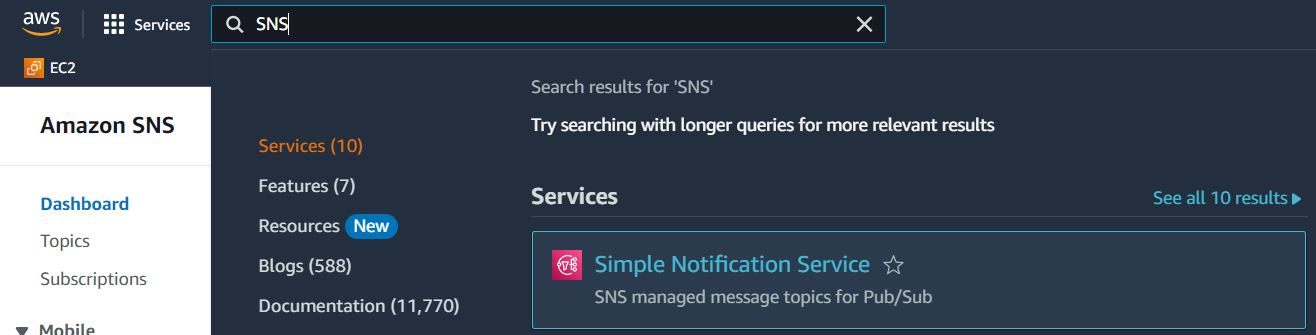
\includegraphics[scale=0.4]{instructions/sns/1.JPG}
  \caption{Създаване на Amazon SNS Topic - стъпка 1.}
\end{figure}

\noindent\textbf{Стъпка 2.} От менюто изберете \textit{Topics}.
\begin{figure}[h!]
\centering
    
\includegraphics[scale=0.55]{instructions/sns/2.JPG}
  \caption{Създаване на Amazon SNS Topic - стъпка 2.}
\end{figure}

\noindent\textbf{Стъпка 3.} Изберете бутона \textit{Create topic}.
\begin{figure}[h!]
\centering
    
\includegraphics[scale=0.6]{instructions/sns/3.JPG}
  \caption{Създаване на Amazon SNS Topic - стъпка 3.}
\end{figure}

\noindent\textbf{Стъпка 4.} В подменюто Type изберете Standard. Попълнете в полето Name име. За целите на текущото ръководство ще използваме \textbf{topic}.
\begin{figure}[h!]
\centering
    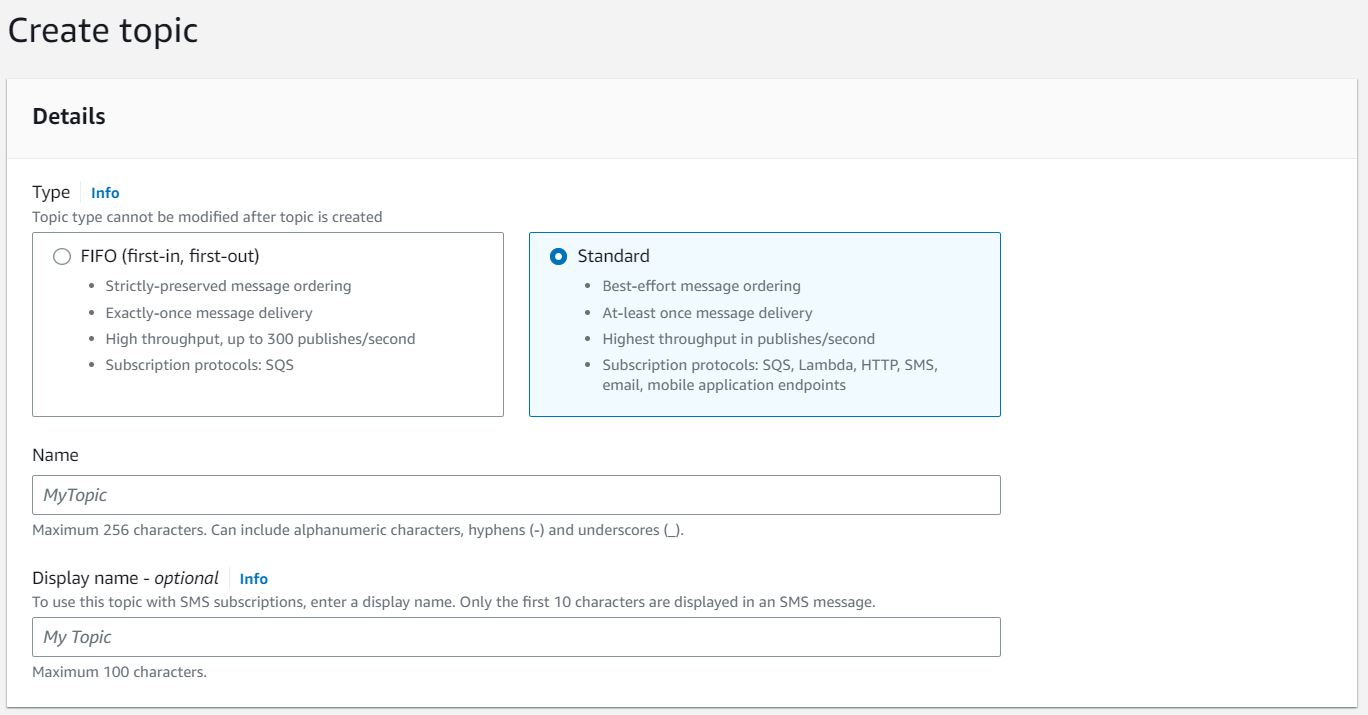
\includegraphics[scale=0.4]{instructions/sns/4.JPG}
  \caption{Създаване на Amazon SNS Topic - стъпка 4.}
\end{figure}

\noindent\textbf{Стъпка 5.} Оставете настройките по подразбиране на останалите опции и изберете бутона \textit{Create topic}.

\noindent\textbf{Стъпка 6.} От менюто изберете \textit{Subscriptions}.
\begin{figure}[h!]
\centering
    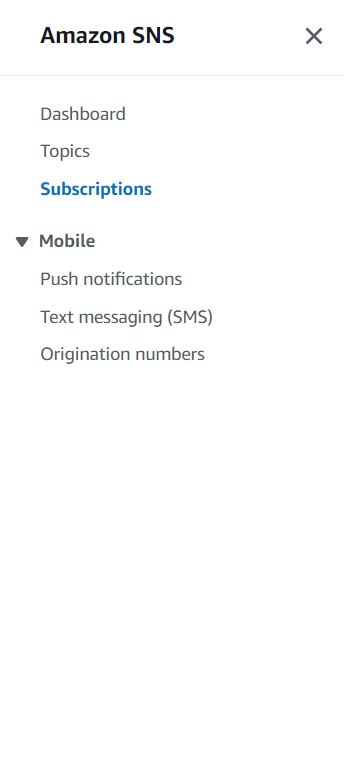
\includegraphics[scale=0.5]{instructions/sns/6.JPG}
  \caption{Създаване на Amazon SNS Topic - стъпка 6.}
\end{figure}

\noindent\textbf{Стъпка 7.} Изберете бутона \textit{Create subscription}.
\begin{figure}[h!]
\centering
    
\includegraphics[scale=0.55]{instructions/sns/7.JPG}
  \caption{Създаване на Amazon SNS Topic - стъпка 7.}
\end{figure}

\noindent\textbf{Стъпка 8.} В Topic ARN изберете ARN на създадения Amazon SNS Topic. В Protocol изберете Email. В полето Endpoint въведете имейл адреса, който да получава известията.
\begin{figure}[h!]
\centering
    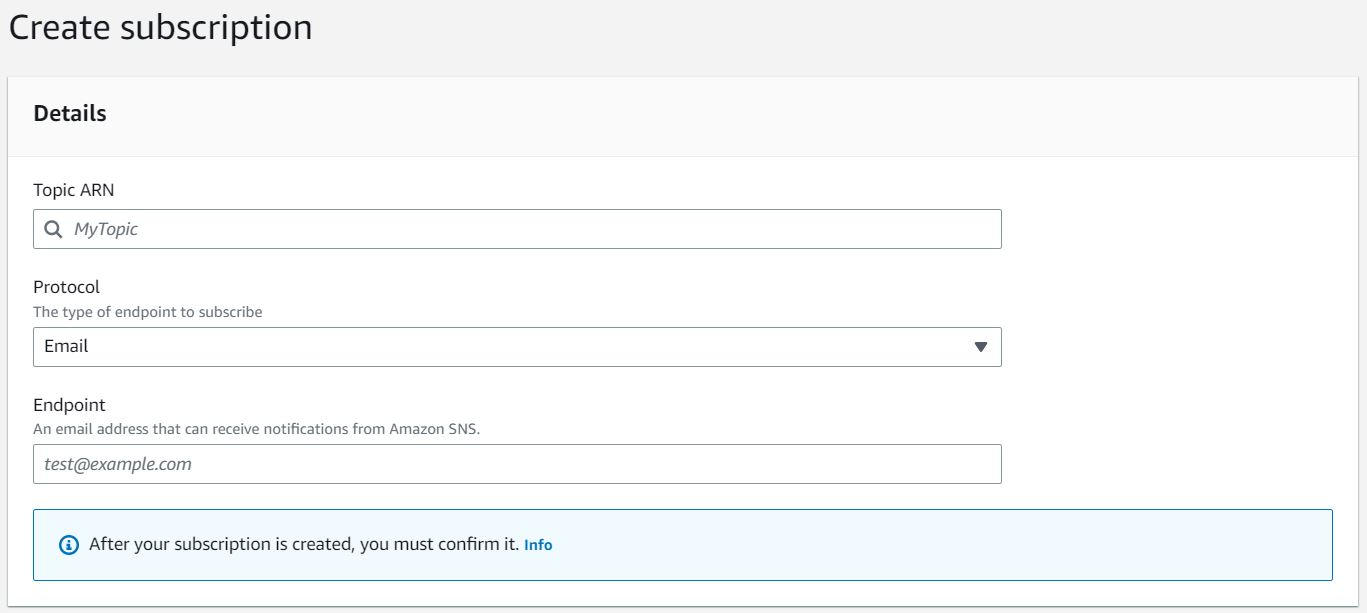
\includegraphics[scale=0.5]{instructions/sns/8.JPG}
  \caption{Създаване на Amazon SNS Topic - стъпка 8.}
\end{figure}

\noindent\textbf{Стъпка 9.} Оставете настройките по подразбиране на останалите опции и изберете бутона \textit{Create subscription}.

\clearpage
\pagebreak

\subsection{Създаване на роли чрез AWS Identity and Access Management (IAM)}
\noindent\textbf{Стъпка 1.} От менюто изберете \textit{Access management > Policies}.
\begin{figure}[h!]
\centering
    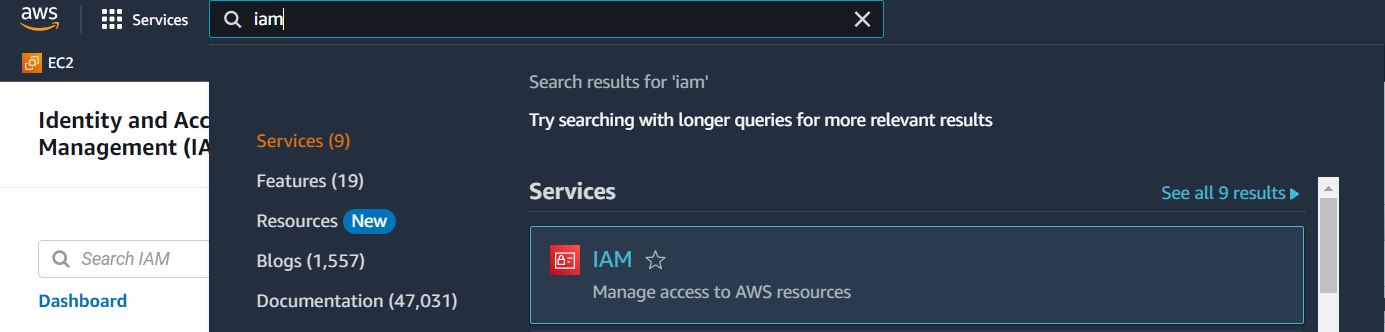
\includegraphics[scale=0.4]{instructions/iam/1.JPG}
  \caption{Създаване на роли чрез AWS IAM - стъпка 1.}
\end{figure}


\noindent\textbf{Стъпка 2.} От менюто изберете \textit{Access management > Policies}.
\begin{figure}[h!]
\centering
    
\includegraphics[scale=0.55]{instructions/iam/2.JPG}
  \caption{Създаване на роли чрез AWS IAM - стъпка 2.}
\end{figure}

\noindent\textbf{Стъпка 3.} Изберете бутона \textit{Create policy}.
\begin{figure}[h!]
\centering
    
\includegraphics[scale=0.7]{instructions/iam/3.JPG}
  \caption{Създаване на роли чрез AWS IAM - стъпка 3.}
\end{figure}

\noindent\textbf{Стъпка 4.} Изберете бутона \textit{JSON}.
\begin{figure}[h!]
\centering
    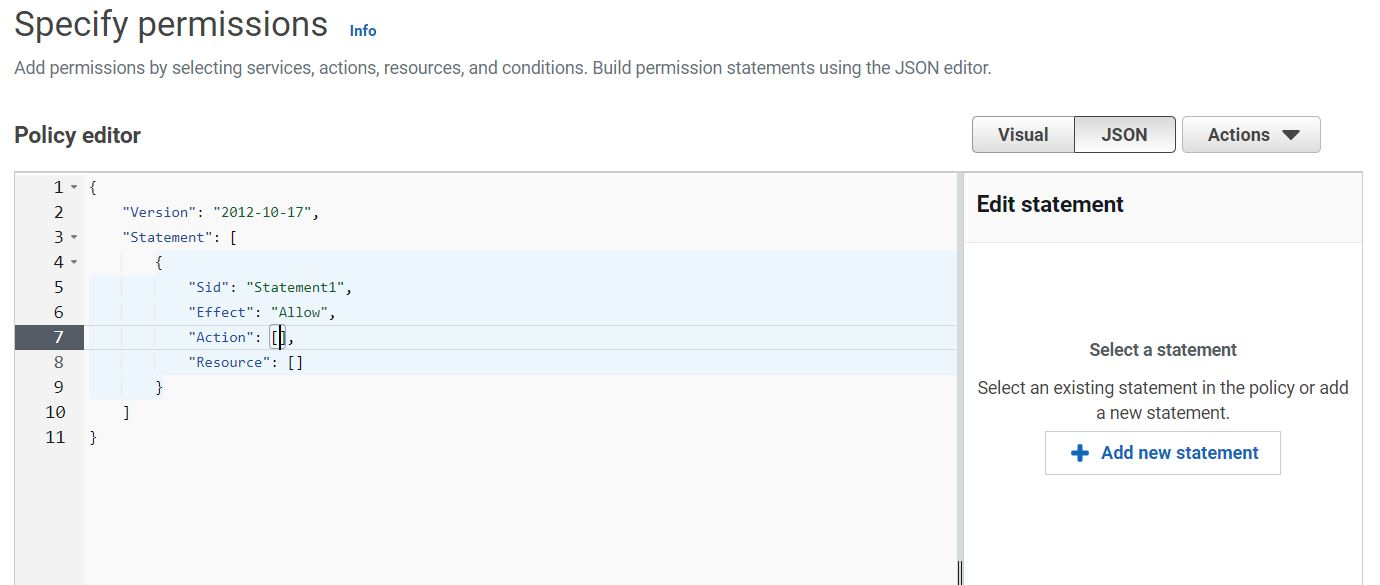
\includegraphics[scale=0.5]{instructions/iam/4.JPG}
  \caption{Създаване на роли чрез AWS IAM - стъпка 4.}
\end{figure}

\noindent\textbf{Стъпка 5.} Заменете съдържанието на Policy editor полето със следния текст, като на местата, означени с коментар, заместите с необходимите данни на създадените в предните стъпки услуги.

\begin{verbatim}
{
    "Version": "2012-10-17",
    "Statement": [
        {
            "Action": [
                "sqs:DeleteMessage",
                "sqs:ListQueues",
                "sqs:ReceiveMessage"
            ],
            "Effect": "Allow",
            "Resource": "" # ARN на Amazon SQS Queue
        },
        {
            "Action": [
                "sns:Subscribe",
                "sns:Publish"
            ],
            "Effect": "Allow",
            "Resource": "" # ARN на Amazon SNS Topic
        },
        {
            "Action": [
                "s3:GetObject",
                "s3:PutObject",
                "s3:ListBucket",
                "s3:PutObjectAcl"
            ],
            "Effect": "Allow",
            "Resource": [
                "", # ARN на основния Amazon S3 Bucket
                "" # ARN на основния Amazon S3 Bucket + "/*"
            ]
        },
        {
            "Action": [
                "dynamodb:CreateTable",
                "dynamodb:PutItem",
                "dynamodb:Update*"
            ],
            "Effect": "Allow",
            "Resource": "" # ARN на Amazon DynamoDB Table
        },
        {
            "Action": [
                "rekognition:DetectLabels"
            ],
            "Effect": "Allow",
            "Resource": "*"
        },
        {
            "Action": [
                "logs:PutLogEvents"
            ],
            "Effect": "Allow",
            "Resource": "*"
        },
        {
            "Effect": "Allow",
            "Action": "logs:CreateLogGroup",
            "Resource": "" # "arn:aws:logs:" + AWS регион + ":" + Account ID + ":*"
        },
        {
            "Effect": "Allow",
            "Action": [
                "logs:CreateLogStream",
                "logs:PutLogEvents"
            ],
            "Resource": [
                "*"
            ]
        }
    ]
}
\end{verbatim}

\noindent\textbf{Стъпка 6.} Изберете бутона \textit{Next}.

\noindent\textbf{Стъпка 7.} Попълнете в полето Policy name име. За целите на текущото ръководство ще използваме \textbf{main-policy}.

\begin{figure}[h!]
\centering
    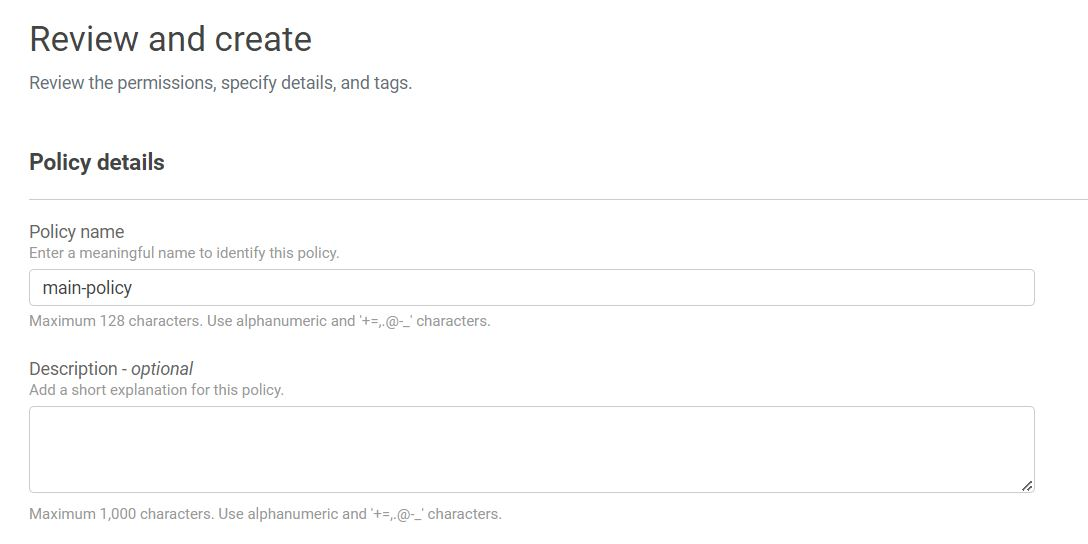
\includegraphics[scale=0.6]{instructions/iam/7.JPG}
  \caption{Създаване на роли чрез AWS IAM - стъпка 7.}
\end{figure}

\noindent\textbf{Стъпка 8.} За да го запазите изберете бутона \textbf{Create policy}.

\noindent\textbf{Стъпка 9.} Повторете отново стъпки 3. до 7., като замените текста с приложения. За целите на текущото ръководство за следващата политика ще използваме името \textbf{dynamodb-s3-policy}.

\begin{verbatim}
{
    "Version": "2012-10-17",
    "Statement": [
        {
            "Action": [
                "dynamodb:CreateTable",
                "dynamodb:PutItem",
                "dynamodb:Update*",
                "dynamodb:Scan"
            ],
            "Effect": "Allow",
            "Resource": "" # ARN на Amazon DynamoDB таблица
        },
        {
            "Action": [
                "s3:PutObject",
                "s3:GetObject"
            ],
            "Effect": "Allow",
            "Resource": [
                "", # ARN на резервния Amazon S3 Bucket
                "" # ARN на резервния Amazon S3 Bucket + "/*"
            ]
        },
        {
            "Action": [
                "logs:PutLogEvents"
            ],
            "Effect": "Allow",
            "Resource": "*"
        },
        {
            "Effect": "Allow",
            "Action": "logs:CreateLogGroup",
            "Resource": "" # "arn:aws:logs:" + AWS регион + ":" + Account ID + ":*"
        },
        {
            "Effect": "Allow",
            "Action": [
                "logs:CreateLogStream",
                "logs:PutLogEvents"
            ],
            "Resource": [
                "*"
            ]
        }
    ]
}
\end{verbatim}


\noindent\textbf{Стъпка 10.} Повторете отново стъпки 3. до 7., като замените текста с приложения. За целите на текущото ръководство за следващата политика ще използваме името \textbf{dynamodb-sns-policy}.

\begin{verbatim}
{
    "Version": "2012-10-17",
    "Statement": [
        {
            "Action": [
                "s3:ListBucket",
                "s3:GetObject",
                "s3:PutObject"
            ],
            "Effect": "Allow",
            "Resource": [
                "", # ARN на резервния Amazon S3 Bucket
                "" # ARN на резервния Amazon S3 Bucket + "/*"
            ]
        },
        {
            "Action": [
                "sns:Subscribe",
                "sns:Publish"
            ],
            "Effect": "Allow",
            "Resource": # ARN на Amazon SNS Topic
        },
        {
            "Action": [
                "logs:PutLogEvents"
            ],
            "Effect": "Allow",
            "Resource": "*"
        },
        {
            "Effect": "Allow",
            "Action": "logs:CreateLogGroup",
            "Resource": "" # "arn:aws:logs:" + AWS регион + ":" + Account ID + ":*"
        },
        {
            "Effect": "Allow",
            "Action": [
                "logs:CreateLogStream",
                "logs:PutLogEvents"
            ],
            "Resource": [
                "*"
            ]
        }
    ]
}
\end{verbatim}


\clearpage
\pagebreak


\subsection{Създаване на Amazon Lambda Function}
\noindent\textbf{Стъпка 1.} Напишете в търсачката "Lambda" и изберете \textit{Lambda} от падащото меню с услуги.
\begin{figure}[h!]
\centering
    \includegraphics[scale=0.4]{instructions/lambda/1.JPG}
  \caption{Създаване на Amazon Lambda Function - стъпка 1.}
\end{figure}

\noindent\textbf{Стъпка 2.} От менюто изберете \textit{Functions}.
\begin{figure}[h!]
\centering
    
\includegraphics[scale=0.55]{instructions/lambda/2.JPG}
  \caption{Създаване на Amazon Lambda Function - стъпка 2.}
\end{figure}

\noindent\textbf{Стъпка 3.} Изберете бутона \textit{Create function}.
\begin{figure}[h!]
\centering
    
\includegraphics[scale=0.6]{instructions/lambda/3.JPG}
  \caption{Създаване на Amazon Lambda Function - стъпка 3.}
\end{figure}

\noindent\textbf{Стъпка 4.} Изберете Author from scratch. Попълнете в полето Function name име. За целите на текущото ръководство ще използваме \textbf{main-lambda}. В Runtime изберете Python 3.8.
\begin{figure}[h!]
\centering
    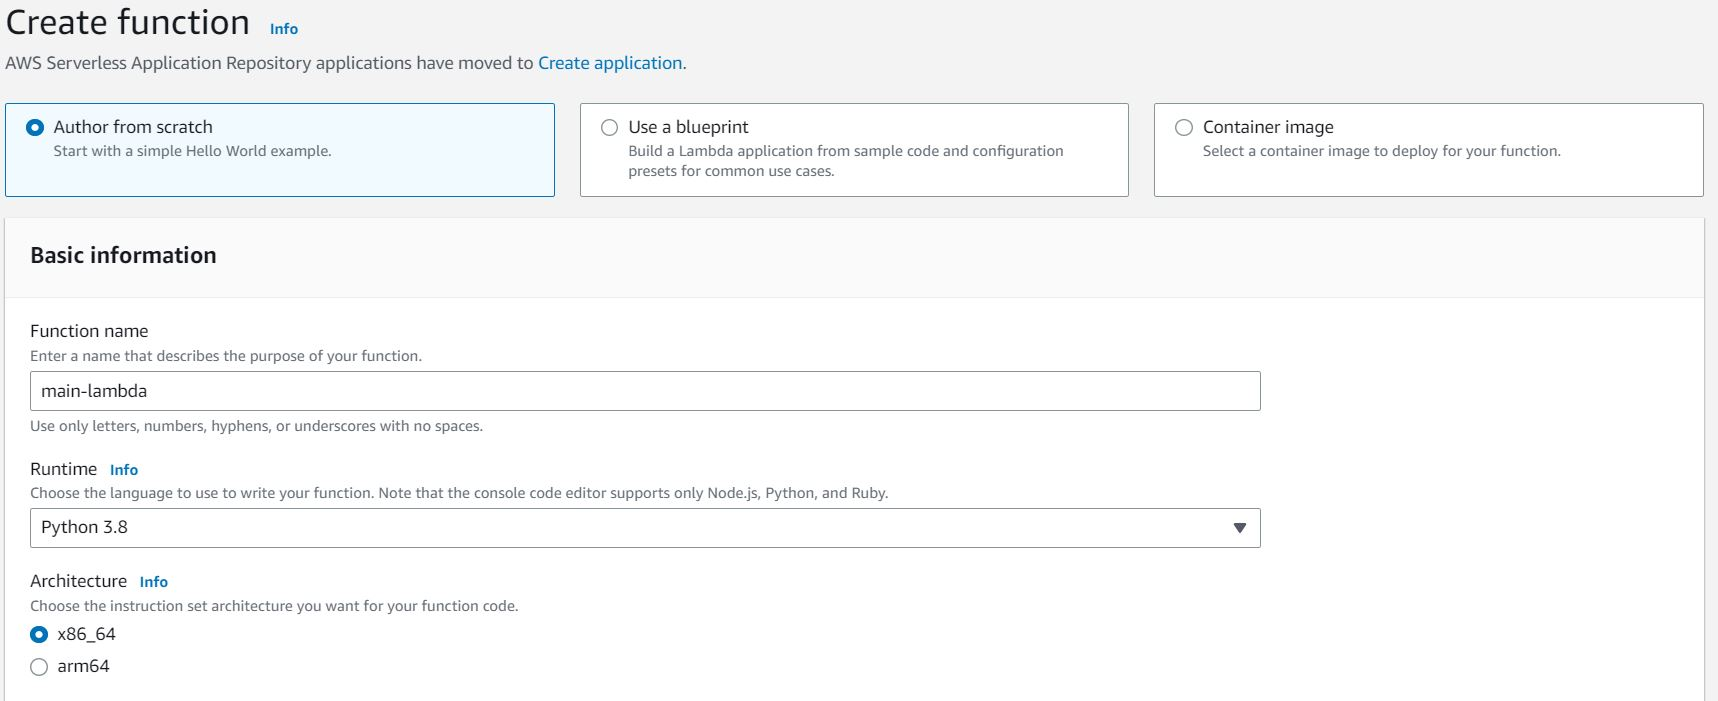
\includegraphics[scale=0.4]{instructions/lambda/4.JPG}
  \caption{Създаване на Amazon Lambda Function - стъпка 4.}
\end{figure}

\noindent\textbf{Стъпка 5.} Изберете Change default execution role. В Execution role изберете Use an existing role. От падащото меню Existing role изберете main-policy. 
\begin{figure}[h!]
\centering
    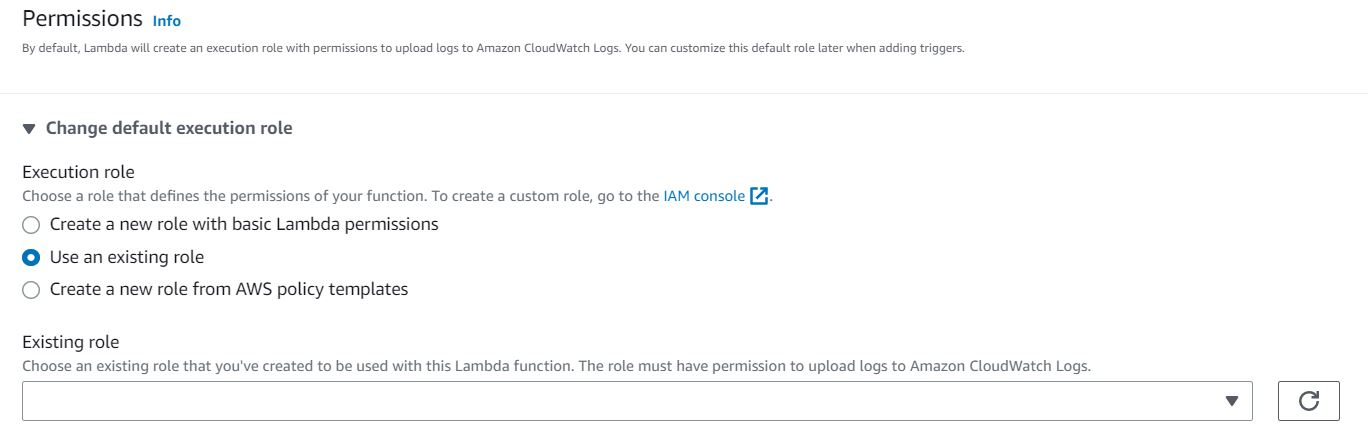
\includegraphics[scale=0.55]{instructions/lambda/5.JPG}
  \caption{Създаване на Amazon Lambda Function - стъпка 5.}
\end{figure}

\noindent\textbf{Стъпка 6.} Оставете настройките по подразбиране на останалите опции и изберете бутона \textit{Create function}.

\noindent\textbf{Стъпка 7.} В полето Code source въведете кода от \ref{subsec-main-lambda}, като на указаните места в декларацията на променливи добавите данните за създадените ресурси. За Amazon S3 Bucket посочете main-bucket.
\begin{figure}[h!]
\centering
    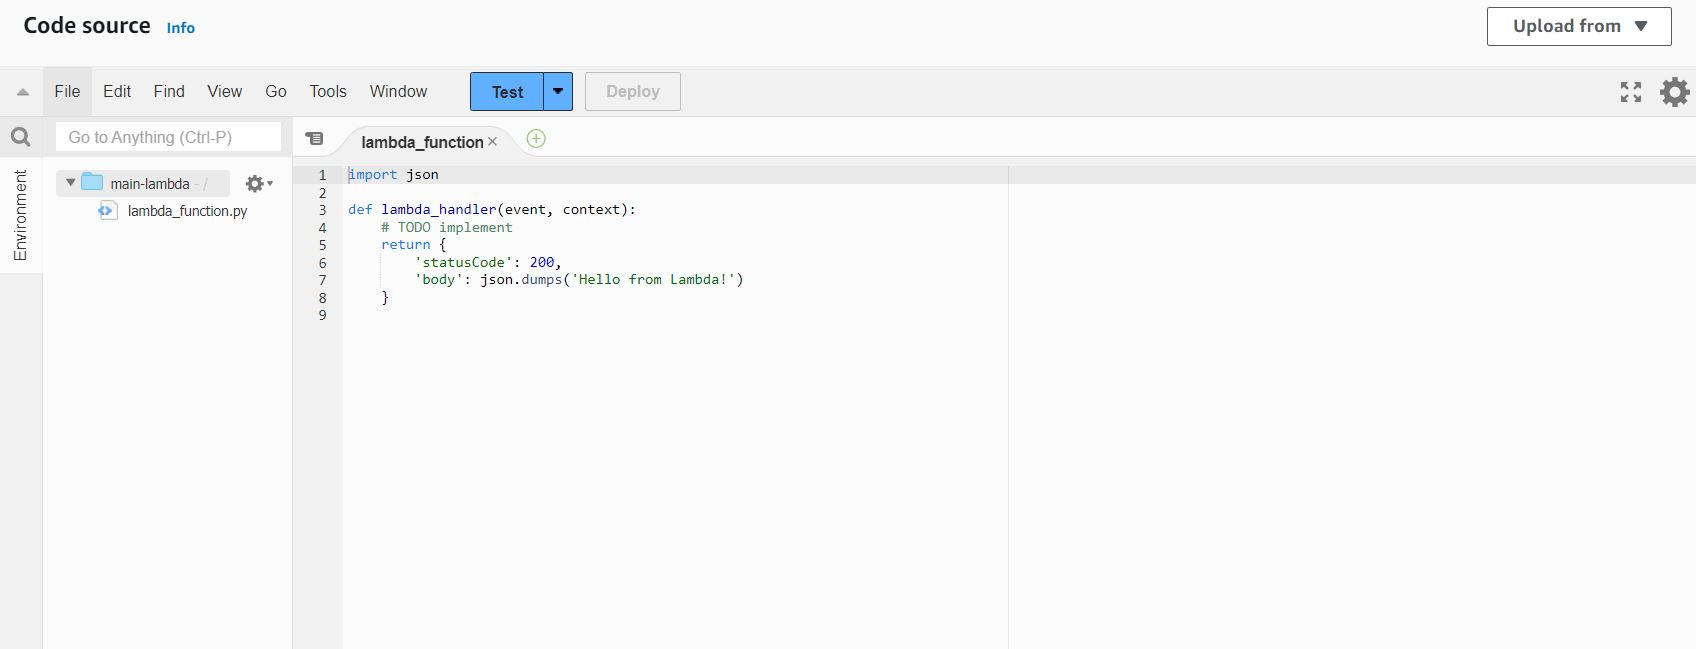
\includegraphics[scale=0.4]{instructions/lambda/7.JPG}
  \caption{Създаване на Amazon Lambda Function - стъпка 7.}
\end{figure}

\noindent\textbf{Стъпка 8.} Изберете бутона \textit{Deploy}.
\begin{figure}[h!]
\centering
    
\includegraphics[scale=0.7]{instructions/lambda/8.JPG}
  \caption{Създаване на Amazon Lambda Function - стъпка 8.}
\end{figure}

\noindent\textbf{Стъпка 9.} Повторете отново стъпки 3. до 8., като използвате dynamodb-s3-policy. В полето Code source въведете кода от \ref{subsec-dynamodb-s3} с Amazon S3 Bucket backup-bucket. За целите на текущото ръководство ще зададем името \textbf{dynamodb-s3-lambda}.

\noindent\textbf{Стъпка 10.} Повторете отново стъпки 3. до 8., като използвате dynamodb-sns-policy. В полето Code source въведете кода от \ref{subsec-dynamodb-sns} с Amazon S3 Bucket backup-bucket. За целите на текущото ръководство ще зададем името \textbf{dynamodb-sns-lambda}.

\clearpage
\pagebreak


\subsection{Създаване на Amazon CloudWatch Rule}
\noindent\textbf{Стъпка 1.} Напишете в търсачката "CloudWatch" и изберете \textit{CloudWatch} от падащото меню с услуги.
\begin{figure}[h!]
\centering
    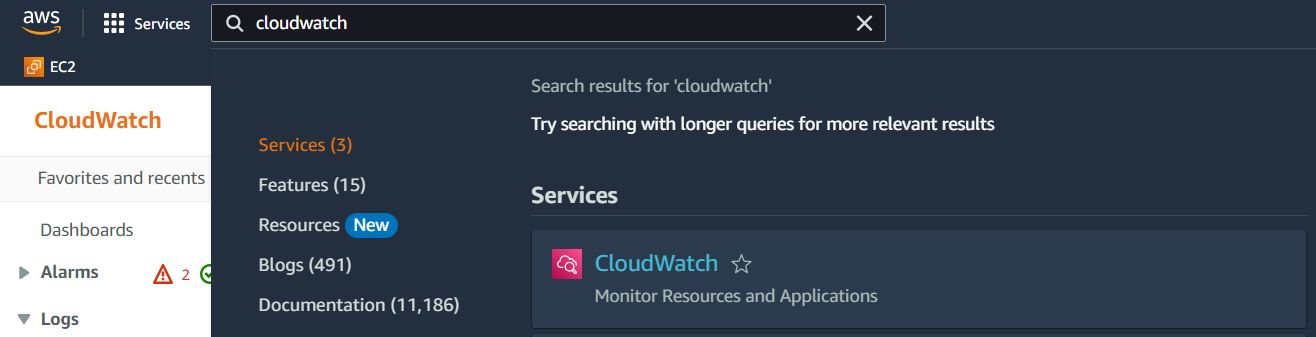
\includegraphics[scale=0.4]{instructions/cloudwatch/1.JPG}
  \caption{Създаване на Amazon CloudWatch Rule - стъпка 1.}
\end{figure}

\noindent\textbf{Стъпка 2.} От менюто изберете \textit{Events > Rules}.
\begin{figure}[h!]
\centering
    
\includegraphics[scale=0.55]{instructions/cloudwatch/2.JPG}
  \caption{Създаване на Amazon CloudWatch Rule - стъпка 2.}
\end{figure}

\noindent\textbf{Стъпка 3.} Изберете бутона \textit{Create rule}.
\begin{figure}[h!]
\centering
    
\includegraphics[scale=0.6]{instructions/cloudwatch/3.JPG}
  \caption{Създаване на Amazon CloudWatch Rule - стъпка 3.}
\end{figure}

\noindent\textbf{Стъпка 4.} Изберете Schedule и в полето Fixed rate of въведете интервала от време, през който искате да се проверява опашката за получени съобщения.
\begin{figure}[h!]
\centering
    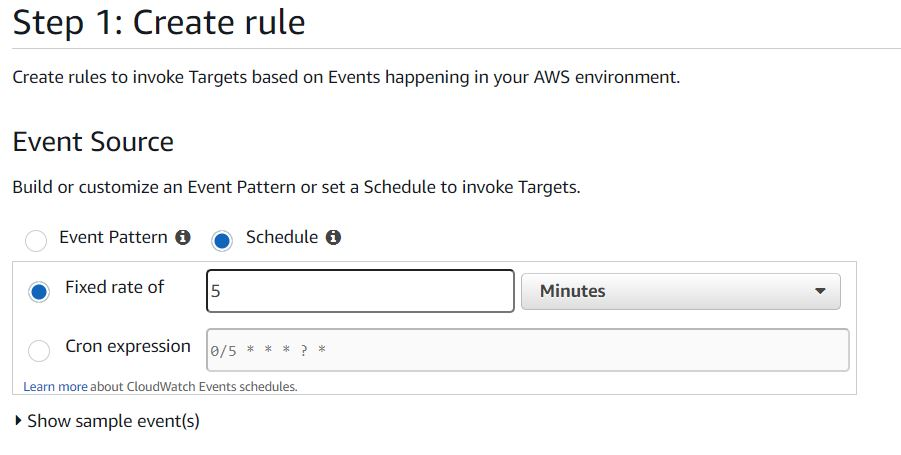
\includegraphics[scale=0.5]{instructions/cloudwatch/4.JPG}
  \caption{Създаване на Amazon CloudWatch Rule - стъпка 4.}
\end{figure}

\noindent\textbf{Стъпка 5.} В Targets изберете бутона Add target. От падащото меню изберете Lambda function, след което от Function посочете main-lambda. 
\begin{figure}[h!]
\centering
    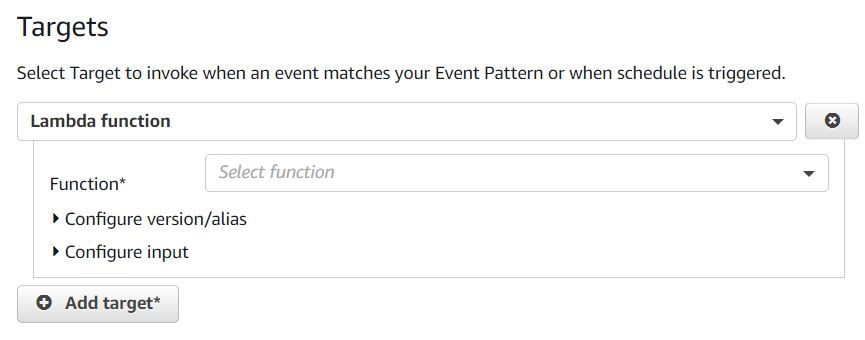
\includegraphics[scale=0.5]{instructions/cloudwatch/5.JPG}
  \caption{Създаване на Amazon CloudWatch Rule - стъпка 5.}
\end{figure}

\noindent\textbf{Стъпка 6.} Оставете настройките по подразбиране на останалите опции и изберете бутона \textit{Configure details}.

\noindent\textbf{Стъпка 7.} В Name въведете име и изберете бутона \textit{Create rule}.
\begin{figure}[h!]
\centering
    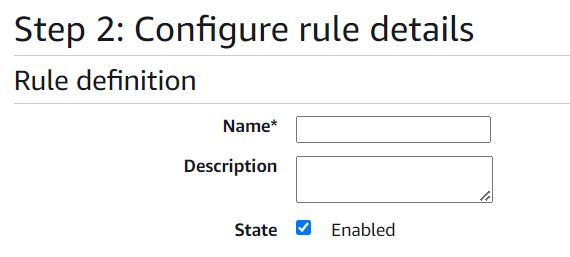
\includegraphics[scale=0.5]{instructions/cloudwatch/7.JPG}
  \caption{Създаване на Amazon CloudWatch Rule - стъпка 7.}
\end{figure}

\noindent\textbf{Стъпка 8.} Повторете отново стъпки 3. до 7., като в Target посочвате всяка от останалите функции.

\clearpage
\pagebreak


\section{Кратко ръководство за потребителя}

\hspace{\parindent}След добавянето на имейл адрес в Amazon SNS Subscription, до него ще бъде изпратено съобщение за потвърждение. За потвърждение е необходимо да се избере \textit{Confirm subscription}.

\begin{figure}[h!]
\centering
    \includegraphics[scale=0.8]{user_guide/1.jpg}
  \caption{Потвъждаване на абонамент към Amazon SNS Subscription.}
\end{figure}

След като абонаментът е потвърден, към този адрес ще започнат да се изпращат съобщения.

\begin{figure}[h!]
\centering
    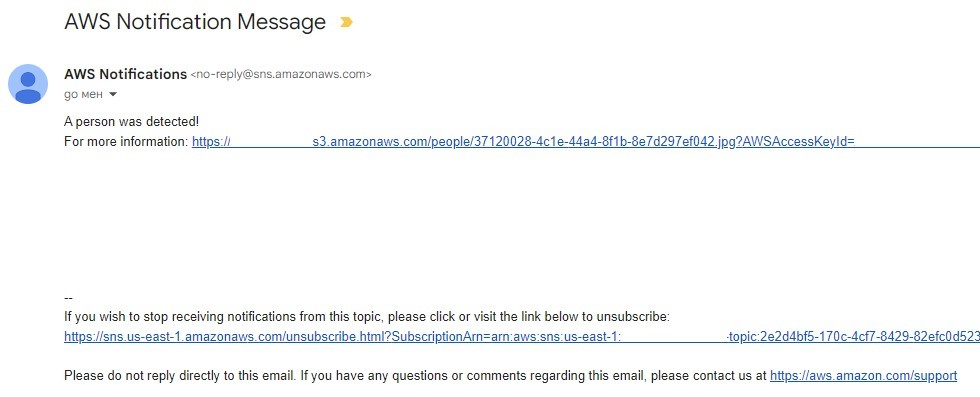
\includegraphics[scale=0.6]{user_guide/4.jpg}
  \caption{Съобщение за откриване на човек на снимката.}
\end{figure}

\begin{figure}[h!]
\centering
    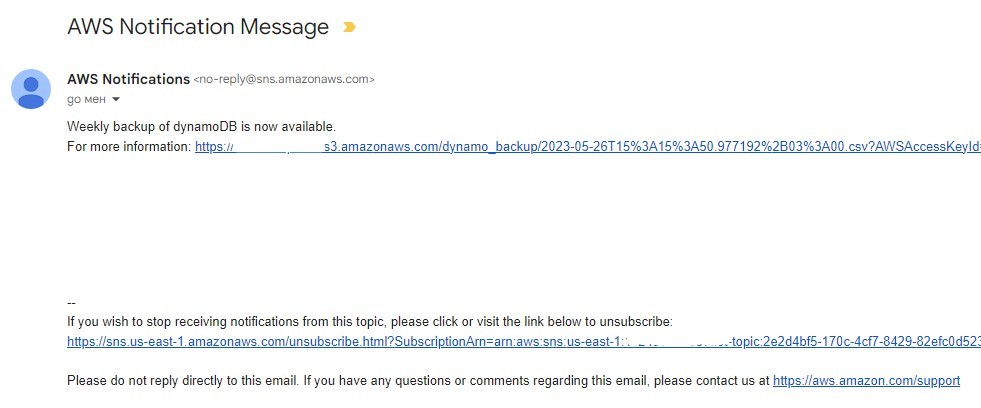
\includegraphics[scale=0.6]{user_guide/3.jpg}
  \caption{Съобщение за готово седмично резервно копие на Amazon DynamoDB Table.}
\end{figure}

За прекратяване на абонамента се използва връзката, предоставена в долната част на получените имейли, като при спиране бива изпратено писмо с потвърждение.

\begin{figure}[h!]
\centering
    
\includegraphics[scale=0.8]{user_guide/2.jpg}
  \caption{Потвъждаване на прекратяването на абонамент към Amazon SNS Subscription.}
\end{figure}

\clearpage
\pagebreak

\section{Примерни данни}

\hspace{\parindent}Демонстрация на работата на системата върху следното изображение:

\begin{figure}[h!]
\centering
    
\includegraphics[scale=0.15]{example_image.jpg}
  \caption{Примерно изображение. [Jake Nackos, Unsplash]}
\end{figure}

Преобразуваме изображението в 64-битов формат. Създаваме JSON файл, в който срещу ключа "encoded\_image" \ записваме кодираната снимка.

\begin{verbatim}
{
    "encoded_img": "/9j/4AAQSkZJRgABAQEASABIAAD<...>KYH/9k="
}
\end{verbatim}

Резултатът от обработката на изображението е показан на приложената диаграма.

\begin{figure}[h!]
\centering
    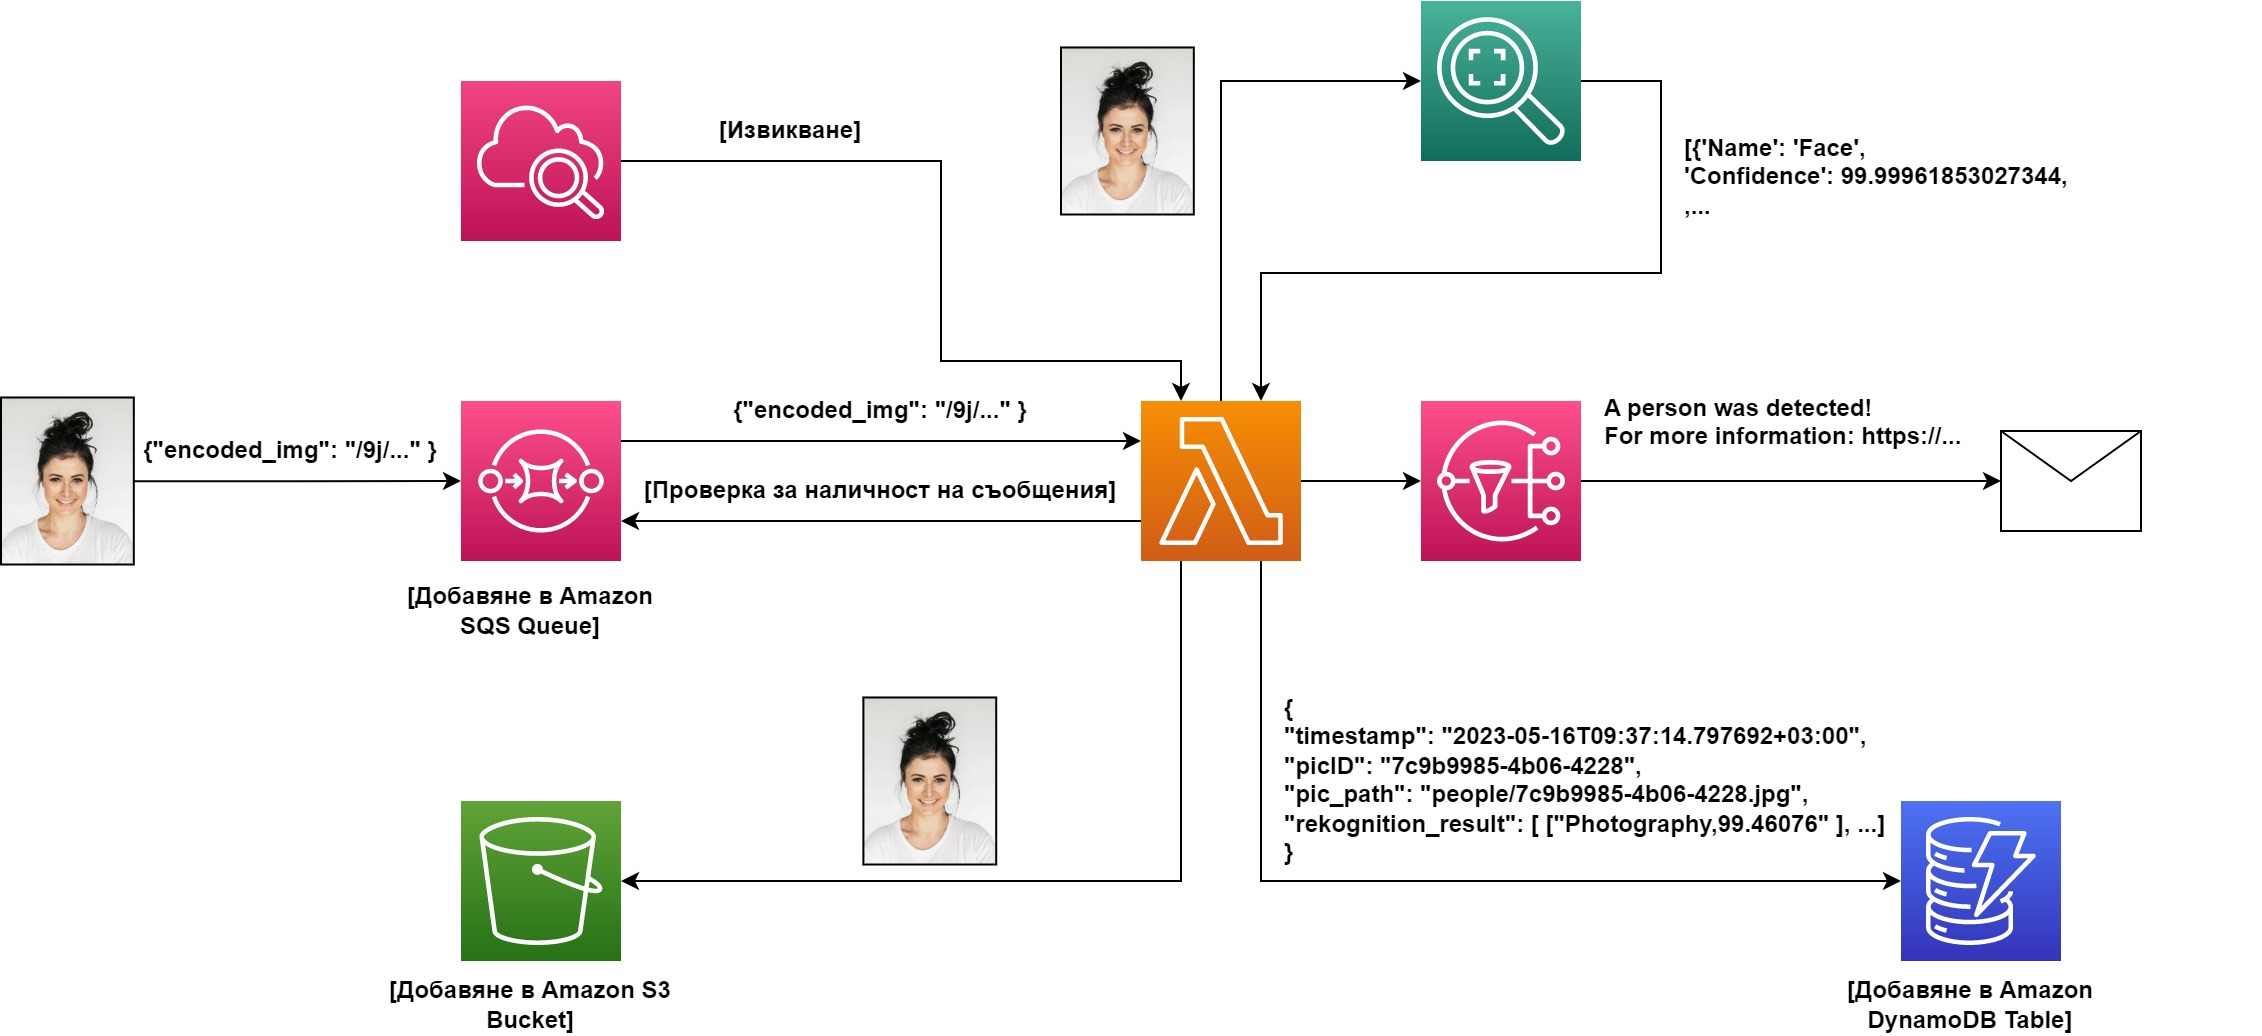
\includegraphics[width=\linewidth]{AWS_example.jpg}
  \caption{Работа на системата с примерни данни. [Diagrams.net]}
\end{figure}

\clearpage
\pagebreak
 
\section{Описание на програмния код}

\hspace{\parindent}За реализирането на логиката в Amazon Lambda Function е използван езикът Python (версия 3.8) и библиотеката boto3.

\subsection{Обработка на получено изображение} \label{subsec-main-lambda}

\hspace{\parindent}Включване на използваните библиотеки:
\begin{verbatim}
import base64
import boto3
from datetime import datetime
import dateutil
import json
import uuid
\end{verbatim}

Деклариране на променливи, съдържащи използваните ресурси:
\begin{verbatim}
QUEUE = '' # URL на Amazon SQS Queue
BUCKET = '' # име на Amazon S3 Bucket
TOPIC = '' # ARN на Amazon SNS Topic
TABLE = '' # име на Amazon DynamoDB Table
REGION = '' # име на Amazon регион
\end{verbatim}

Функция, връщаща получените от Amazon SQS опашката с URL стойността на QUEUE съобщения:
\begin{verbatim}
def get_messages():
    return boto3.client(
        'sqs',
        region_name=REGION
    ).receive_message(
        QueueUrl=QUEUE,
        MaxNumberOfMessages=1
    )
\end{verbatim}

Функция, премахваща от опашката съобщение:
\begin{verbatim}
def delete_message(receipt_handle):
    return boto3.client(
        'sqs',
        region_name=REGION
    ).delete_message(
        QueueUrl=QUEUE,
        ReceiptHandle=receipt_handle
    )
\end{verbatim}

Функция, създаваща временен файл със съдържание снимката, получена в опашката:
\begin{verbatim}
def write_picture(sqs_messages):
    pic_uuid = str(uuid.uuid4())
    pic_path = f'/tmp/{pic_uuid}.jpg'

    decoded_image = base64.b64decode(
        json.loads(
            sqs_messages['Messages'][0]['Body']
        )['encoded_img']
    )

    with open(pic_path, 'wb') as f:
        f.write(decoded_image)

    return pic_uuid, pic_path
\end{verbatim}

Функция, извикваща Amazon Recognition върху подадена снимка, и връщаща 10-те етикета, получени с най-голяма вероятност:
\begin{verbatim}
def run_rekognition(pic_path):
    with open(pic_path, 'rb') as image:
        return boto3.client(
            'rekognition',
            region_name=REGION
        ).detect_labels(
            Image={
                'Bytes': image.read()
            },
            MaxLabels=10,
        )['Labels']
\end{verbatim}

Функция, проверяваща дали Amazon Rekognition е поставил на етикета "човек" \ вероятност, по-голяма от 90\%, и той е сред десетте разпознати с най-голяма вероятност обекти на снимката:
\begin{verbatim}
def detect_person(pic_path):
    rekognition_labels = run_rekognition(pic_path)

    is_person = False
    for label in rekognition_labels:
        label_name = label['Name'].lower()
        label_confidence = label['Confidence']

        if label_name in ['human', 'person'] and label_confidence >= 90:
            is_person = True
    return is_person, rekognition_labels
\end{verbatim}

Функция, добавяща към Amazon DynamoDB таблицата TABLE нов запис, съдържащ инфомация за снимката и резултата, получен от Amazon Rekognition:
\begin{verbatim}
def add_to_dynamoDB(pic_uuid, labels, pic_path):
    table = boto3.resource(
        'dynamodb',
        region_name=REGION
    ).Table(TABLE)

    table.put_item(
        Item={
            'timestamp': str(datetime.now(
                            dateutil.tz.gettz('Europe/Sofia')
                        ).isoformat()),
            'picID': pic_uuid,
            'pic_path': pic_path,
            'rekognition_result': [
                ','.join([label['Name'], str(label['Confidence'])])
                for label
                in labels
            ]
        }
    )
\end{verbatim}

Функция, добавяща в Amazon S3 Bucket с име BUCKET подаденото като параметър изображение:
\begin{verbatim}
def add_to_bucket(img, pic_path):
    boto3.client(
        's3',
        region_name=REGION
    ).upload_file(
        img,
        BUCKET,
        pic_path
    )
\end{verbatim}

Функция, генерираща валиден 24 часа URL към обект, съхранен в Amazon S3:
\begin{verbatim}
def get_public_url(file):
    return boto3.client(
        's3',
        region_name=REGION
    ).generate_presigned_url(
        ClientMethod='get_object',
        Params={
            'Bucket': BUCKET,
            'Key': file
        },
        ExpiresIn=86400
    )
\end{verbatim}

Функция, публикуваща в TOPIC ново съобщение, съдържащо публичен линк към снимката, подадена като параметър: 
\begin{verbatim}
def publish_to_topic(img_path):
    boto3.client(
        'sns',
        region_name=REGION
    ).publish(
        TopicArn=TOPIC,
        Message=f'A person was detected!'
                f'\nFor more information: {get_public_url(img_path)}'
    )
\end{verbatim}

Основна функция, която получава всички съобщения в Amazon SQS опашката. Ако такива са налични, започва обработката на едно от тях. Проверява дали на снимката от текущото съобщение има човек, и, ако това е така, запазва снимката в Amazon S3 пространството за съхранение, добавя информацията за нея в Amazon DynamoDB таблицата и изпраща съобщение към Amazon SNS услугата. При завършване на работата с текущото изображение го премахва от опашката:
\begin{verbatim}
def lambda_handler(event, context):
    sqs_messages = get_messages()

    if "Messages" in sqs_messages:
        pic_uuid, pic_path = write_picture(sqs_messages)
        is_person, rekognition_labels = detect_person(pic_path)

        if is_person:
            saved_pic_path = pic_path.replace("/tmp/", "people/")
            add_to_dynamoDB(
                pic_uuid=pic_uuid,
                pic_path=saved_pic_path,
                labels=rekognition_labels
            )
            add_to_bucket(
                img=pic_path,
                pic_path=saved_pic_path
            )
            publish_to_topic(
                saved_pic_path
            )
        delete_message(sqs_messages['Messages'][0]['ReceiptHandle'])
    else:
        print("No pictures in queue")

\end{verbatim}

\clearpage
\pagebreak


\subsection{Експортиране на Amazon DynamoDB таблица в CSV формат} \label{subsec-dynamodb-s3}

\hspace{\parindent}Включване на използваните библиотеки:
\begin{verbatim}
import boto3
import csv
from datetime import datetime
import dateutil
\end{verbatim}

Деклариране на променливи, съдържащи използваните ресурси:
\begin{verbatim}
BUCKET = '' # име на Amazon S3 Bucket
TABLE = '' # име на Amazon DynamoDB Table
TEMP_LOCATION = '' # адрес на временния CSV файл
REGION = '' # име на Amazon регион
\end{verbatim}

Функция, извличаща данните от Amazon DynamoDB таблицата:
\begin{verbatim}
def scan_table(previous_response=None):
    table = boto3.resource(
        'dynamodb',
        region_name=REGION
    ).Table(
        TABLE
    )

    if previous_response is not None:
        return table.scan(
            ExclusiveStartKey=previous_response['LastEvaluatedKey']
        )
    else:
        return table.scan()
\end{verbatim}

Функция, добавяща експортираната в CSV формат Amazon DynamoDB таблица в Amazon S3, като за име на файла се използва текущото време:
\begin{verbatim}
def add_to_bucket():
    boto3.resource(
        's3',
        region_name=REGION
    ).Bucket(
        BUCKET
    ).upload_file(
        TEMP_LOCATION,
        'dynamo_backup/' + str(
            datetime.now(
                dateutil.tz.gettz('Europe/Sofia')
            ).isoformat()
        ) + '.csv'
    )
\end{verbatim}

Основна функция, изличаща и записваща в CSV файл записите от Amazon DynamoDB таблицата, и добавяща получения файл в Amazon S3:
\begin{verbatim}
def lambda_handler(event, context):
    with open(TEMP_LOCATION, 'w') as output_file:
        writer = csv.writer(output_file)
        is_start = True

        response = {'LastEvaluatedKey': []}

        while 'LastEvaluatedKey' in response:
            if is_start:
                response = scan_table()
            else:
                response = scan_table(response)
            for item in response['Items']:
                if is_start:
                    writer.writerow(item.keys())
                is_start = False
                writer.writerow(item.values())

    add_to_bucket()
\end{verbatim}

\clearpage
\pagebreak

\subsection{Уведомяване на потребителите за налични CSV файлове} \label{subsec-dynamodb-sns}

\hspace{\parindent}Включване на използваните библиотеки:
\begin{verbatim}
import boto3
\end{verbatim}

Деклариране на променливи, съдържащи използваните ресурси:
\begin{verbatim}
BUCKET = '' # име на Amazon S3 Bucket
TOPIC = '' # ARN на Amazon SNS Topic
REGION = '' # име на Amazon регион
\end{verbatim}

Получаване на последния добавен в Amazon S3 пространството за съхранение CSV файл:
\begin{verbatim}
def last_updated_file():
    paginator = boto3.client(
        's3'
    ).get_paginator(
        "list_objects_v2"
    ).paginate(
        Bucket=BUCKET
    )
    
    result = None
    for page in paginator:
        if "Contents" in page:
            obj = sorted(
                page['Contents'],
                key=lambda x: x['LastModified']
            )[-1]
            if result is None or obj['LastModified'] > result['LastModified']:
                result = obj
    return result['Key']
\end{verbatim}

Функция, генерираща валиден 24 часа URL към обект, съхранен в Amazon S3:
\begin{verbatim}
def get_public_url(file):
    return boto3.client(
        's3',
        region_name=REGION
    ).generate_presigned_url(
        ClientMethod='get_object',
        Params={
            'Bucket': BUCKET,
            'Key': file
        },
        ExpiresIn=86400
    )
\end{verbatim}

Функция, публикуваща в TOPIC ново съобщение, съдържащо публичен линк към снимката, подадена като параметър: 
\begin{verbatim}
def publish_to_topic(img_path):
    boto3.client(
        'sns',
        region_name=REGION
    ).publish(
        TopicArn=TOPIC,
        Message=f'Weekly backup of dynamoDB is now available.'
                f'\nFor more information: {get_public_url(img_path)}'
    )
\end{verbatim}

Основна функция, изпращаща съобщение към Amazon SNS Topic. Съобщението съдържа валиден 24 часа URL за достъп до последния обновен файл в Amazon S3 Bucket:
\begin{verbatim}
def lambda_handler(event, context):
    file_key = last_updated_file()
    publish_to_topic(file_key)
\end{verbatim}

\medskip

\clearpage
\pagebreak

\section{Приноси на студента, ограничения и възможности за бъдещо развитие}

\hspace{\parindent}Поради ограничения при правата за достъп, някои от функционалностите не са налични чрез Amazon Academy. В следстие на това, използваните ресурси са съобразени с квотите в AWS Free Tier.

Потенциална посока за бъдещо развитие на проекта е добавяне на възможност за лицево разпознаване - потребителите могат да добавят своя снимка. При получаване на изображение с човек, лицата да биват сравнявани (напр. чрез използването на инструмент като DeepFace или чрез Amazon Rekognition) и на потребителя да се изпраща съобщение само ако на снимката не е бил разпознат той. Подобно разширение би могло да намери приложение при охранителните камери.

Възможност за разширяване на функционалността на проекта е използване на инструментите, предоставени от Amazon SageMaker, за автоматизация на анализа на събраните данни.

\medskip

\clearpage
\pagebreak

\section{Какво научих}

\hspace{\parindent}Работата по текущия проект е първият ми опит със създаването Cloud-базирано решение. По време на работата успях да се запозная по-обстойно с разгледаните по време на лекциите Amazon услуги.

Създаването на потребителски роли, които отговарят на Least Privilege принципа, и които осигуряват необходимото ниво на сигурност с оглед на съхранението на лични снимки, ми помогна да разбера една от по-непознатите за мен услуги - AWS IAM.

В процеса на работа имах възможността да се запозная с някои от услугите, предлагани от AWS, които не попадат в обхвата на курса - Amazon Rekognition.


\clearpage
\pagebreak

\section{Списък с фигури и таблици}

\listoffigures

\section{Използвани източници}

\noindent\href{https://boto3.amazonaws.com/v1/documentation/api/latest/index.html}{[1] Boto3 documentation}

\noindent\href{https://www.dynamodbguide.com/}{[2] DynamoDB, explained.}

\noindent\href{https://docs.aws.amazon.com/rekognition/latest/dg/images-s3.html}{[3] Analyzing images stored in an Amazon S3 bucket}

\noindent\href{https://awstip.com/aws-rekognition-using-lambda-with-sqs-and-sns-part-1-ca66c37dad7e}{[4] AWS Rekognition using Lambda with SQS and SNS. Part 1 (step by step tutorial)}

\noindent\href{https://medium.com/thelorry-product-tech-data/building-a-simple-scheduled-task-with-aws-using-lambda-function-and-amazon-cloudwatch-event-e92e5e2418cf}{[5] Building a Simple Scheduled Task with AWS using Lambda Function and Amazon Cloudwatch Event}

\noindent\href{https://docs.aws.amazon.com/AmazonS3/latest/userguide/ShareObjectPreSignedURL.html}{[6] Sharing objects using presigned URLs}
 
\medskip


\end{document}